\subsection{Concurrent connection setups}
In order to better understand how the performance of Bluetooth is affected by the load of the network, we developed a test measuring the time required to open two connections on the same device at nearly the same time.
The test involved three devices, two of which opened a Bluetooth connection with the other one nearly at the same time, as shown in Fig. \ref{figure:collision}

\begin{figure}[ht!]
  \centering
  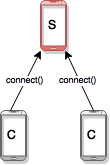
\includegraphics[width=0.2\textwidth]{application/img/collision.png} 
  \caption{To test the time required to open a connection in a loaded network, two client devices connected to a server device at the same time}
  \label{figure:collision}
\end{figure}

\subsubsection{Test execution}
The test has been run \dots times, using \dots different sets of devices.
To start the test a script were executed, that instructed the clients to start a connection with the server and waited for the responses, which included the measurements taken.
In order to limit the time difference at which each of the two clients started the connection, the request made by the script included a time offset that the clients should wait before initializing the connection.